\section{Evaluation}

We evaluate our proposed methods on two different connectomics datasets, one anisotropic and the other isotropic, from two different species. 

\subsection{Datasets}

\subsubsection{Kasthuri}
The Kasthuri dataset images the neocortex of a mouse brain produced by a scanning electron microscope \cite{kasthuri2015saturated}. 
This dataset is $338 \times 3618 \times  5342$ voxels in size. 
The resolution of the dataset is $3 \times 3 \times 30 \textrm{nm}^3$. 
We evaluate our methods using the left cylinder of this 3-cylinder dataset. 

\subsubsection{FlyEM}

The FlyEM dataset comes from the mushroom body of a 5-day old adult male \textit{Drosophila} fly imaged by a focused ion-beam milling scanning electron microscopy.  
The mushroom body is this species is the major site of associative learning \cite{takemura2017connectome}. 
The original dataset contains a $40 \mu\textrm{m} \times 50\mu\textrm{m} \times 120\mu\textrm{m}$ volume of which we use two subsections of size $1000 \times 1000 \times 1000$ voxels.  
The resolution of this dataset is $10 \times 10 \times 10 \mu\textrm{m}^3$ per voxel. 
The image data and the accompanying ground truth is available (CITE). 

\subsubsection{Segmentation Pipeline and Baseline}

Our algorithm takes the output of a supervoxel based agglomeration strategy such as NeuroProof or GALA. For our experiments we use the output from NeuroProof (CITE). We generate voxel affinities from the raw image data using the U-Net architecture \cite{ronneberger2015u}. The Zwatershed algorithm (CITE) creates an oversegmentation of the neurons given these voxel affinities. We input the raw image data, the voxel affinities, and the oversegmentation into NeuroProof which performs a hierarchical agglomeration strategy to merge the supervoxels into larger and larger segments. Two neighboring segments receive a merge-likelihood score based on various extracted features such as the distribution of affinities along the segment boundary. A random forest classifier generates probabilities based on these features. (TODO: TOUFIQ ADD HERE)



\subsection{Skeleton Pruning}

Our method prunes potential merge candidates by considering the skeleton as a simplification of the segment shape. Segment skeletons that have nearby endpoints are merge candidates. The underlying assumption in this model is that the segments break in a particular fashion, primarily perpendicular to the direction of travel (CONFUSING). We perform a series of experiments to evaluate the effectiveness of this idea. First, we examine how many merge candidates are not considered using our method that would have been if we employed the strategy of considering all neighboring segments. These are locations that we cannot possibly correct and therefore we want this number to be as low as possible. The second experiment considers how many locations are not considered that should not be merged. We want this number to be as large as possible since we want to avoid making mistakes by merging these segments. At best, these segments waste time and at worst they lead to incorrect merges. 

\subsection{Classifier Training}

We divide both datasets into half to train the classifier. We generate all valid examples for merge consideration based on the skeletonization algorithm. In the training dataset, $80\%$ of the examples are used for training and the remaining examples are used for validation. To start, we consider networks of varying sizes, optimization functions, and loss functions. The supplemental material has additional information concerning the tuning of the network. There are XXX,XXX learnable parameters in our final architecture. The training ran for XX epochs. Table \ref{table:architecture} provides the final network parameters.

\begin{table}[h!]
	\centering
	\begin{tabular}{l l} \hline
		\textbf{Parameters} & \textbf{Values} \\ \hline
		Loss Function & Mean Squared Error \\
		Optimizer & SGD  with Nesterov Momentum \\
		Momentum & 0.9 \\
		Initial Learning Rate & 0.01 \\
		Decay Rate & $5 * 10^{-8}$ \\
		Activation & LeakyReLU $(\alpha = 0.001)$ \\
		Kernel Sizes & $3 \times 3 \times 3$ \\
		Filter Sizes & $16 \to 32 \to 64$ \\ \hline
	\end{tabular}
	\caption{The parameters for the trained neural network.}
	\label{table:architecture}
\end{table}

\paragraph{Data Augmentation.}
We apply some data augmentation to the generated examples to increase the size of the training datasets. 
We consider all rotations of $90$ degrees along the $xy$-plane in addition to mirrors along the $x$ and $z$ axes. 
This produces an additional 16 times more training data. 

\subsection{Graph-based Strategies}

\begin{figure}
	\centering
	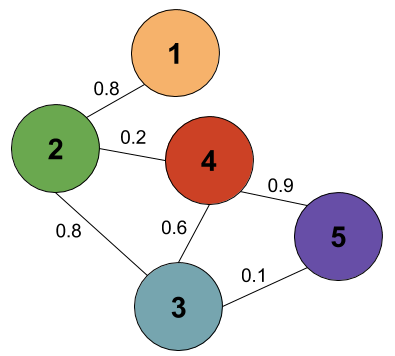
\includegraphics[width=0.8\linewidth]{./figures/multicut.png}
	\caption{An example of the benefits of using multicut over simpler agglomeration schemes. If we input this example into a na\"ive agglomeration strategy that collapses all edges with a threshold greater than 0.5, this entire segment will merge together despite the fact that nodes 2 and 4 and nodes 3 and 5 have low affinities.}
	\label{fig:multicut}
\end{figure}

Most current agglomeration strategies in connectomics consider all pairs of neighboring segments. A classifier produces a probability that each pair belongs to the same segment. All segment pairs with a probability above a certain threshold are merged together. Consider the simple example in Figure \ref{fig:multicut}. Under the existing agglomeration schemes this entire graph would become one segment. However multicut eliminates all cycles within the graph creating two unique segments. We compare our results using both the traditional hierarchical agglomeration strategy with the graph-based approach we propose. 

\subsection{Variation of Information}

We use the variation of information metric to determine the accuracy of our pipeline. The variation of information measures the distance between two segmentations and is similar to mutual information. A lower variation of information score corresponds to a segmentation closer to the ground truth. (TODO: TOUFIQ ADD HERE)

%We evaluate our method on two different connectomics datasets of different species. 

%\subsection{Datasets}

%\subsubsection{Kasthuri}

%The first dataset is the left part of the mouse cortex volume of Kasthuri et al. (CITE). We divide the dataset into a training and validation half and a testing half. The dataset resolution is $3 \times 3 \times 30 \textrm{nm}^3/\textrm{voxel}$. 

%\subsubsection{FlyEM}



%We evaluate our methods on three EM datasets. 
%TODO: Toufiq: add description of the EM datasets (volume size, resolution, type of animal, type of image scan)

%\subsubsection{NeuroProof Pipeline}
%\label{sec:neuroproof}
%Our methods build on top of existing agglomeration strategies. For the purpose of this paper we used the outputs from two established pipelines. 
%TODO: Toufiq description of neuroproof pipeline, description of FlyEM pipeline

%\subsection{Preprocessing}

%We perform significant pruning of potential merge candidates by considering only pairs of skeleton endpoints produced by Algorithm \ref{alg:generate-edges}. This strategy greatly reduced the number of false merge candidates that we considered. However, we evaluate the overall effectiveness of this strategy both in reducing trivial split candidates while maintaining a large majority of the candidates which should merge.

%Our candidate generation strategy doesn't enforce an adjacency constraint which allows us to merge candidates that are not consider under existing frameworks. We examine the success of our pipeline in merging said candidates. 

%\subsection{Classifier Training}

%DISCUSS PARAMETERS FOR CLASSIFICATION

%\subsection{Graph Optimization}

%We evaluate the improvement of using a graph optimization strategy over a na\"ive approach that performs hierarchical clustering for all segments above a certain threshold.
%Using a heuristic for multicut prevents the creation of cycles. 
%Using a simple agglomeration strategy generates this many cycles. 